\chapter{Individuazione tecnologica per il progetto}

\section{Confronto vendors}
Nel mercato sono presenti diversi tipi di soluzioni DLP. Ogni vendor propone il suo prodotto che fa 
concorrenza agli altri. Attraverso un'analisi di mercato sarà più semplice capire quali sono le funzionalità
fondamentali che contraddistinguono una soluzione DLP.

La seguente lista elenca alcuni dei principali prodotti presenti sul mercato:

\begin{itemize}
    \item Endpoint Protector by \textbf{CoSoSys}
    \item \textbf{Digital Guardian} Endpoint DLP
    \item \textbf{Symantec} Data Loss Prevention
    \item \textbf{Comodo} MyDLP
    \item \textbf{Forcepoint} Data Loss Prevention
    \item \textbf{SecureTrust} Data Loss Prevention
    \item \textbf{McAfee} Total Protection for Data Loss Prevention
    \item \textbf{Check Point} Data Loss Prevention
    \item \textbf{Safetica} Data Loss Prevention
  \end{itemize}

  Per lo studio di mercato prenderemo in causa i primi cinque della lista. 
  La tabella \ref{tabellaVendor} mostra similitudini e differenze delle caratteristiche possedute dai 
  principali prodotti DLP.

  \begin{table}[htp]
    \centering
    \resizebox{\textwidth}{!}{%
    \begin{tabular}{|l|c|c|c|c|c|}
    \hline
     &
      \textbf{\begin{tabular}[c]{@{}c@{}}Endpoint \\ Protector\end{tabular}} &
      \textbf{\begin{tabular}[c]{@{}c@{}}Digital\\ Guardian\end{tabular}} &
      \textbf{Symantec} &
      \textbf{MyDLP} &
      \textbf{Forcepoint} \\ \hline
    \rowcolor[HTML]{EFEFEF} 
    {\color[HTML]{333333} \textbf{\begin{tabular}[c]{@{}l@{}}Dati in Transito\\ Network\end{tabular}}} &
      {\color[HTML]{333333} } &
      {\color[HTML]{333333} } &
      {\color[HTML]{333333} } &
      {\color[HTML]{333333} } &
      {\color[HTML]{333333} } \\ \hline
    Traffico Web                                                                                                 & x & x & x & x & x \\ \hline
    Traffico Email                                                                                               & x & x & x & x & x \\ \hline
    Traffico IM                                                                                                  & x &   & x & x & x \\ \hline
    \rowcolor[HTML]{EFEFEF} 
    \textbf{\begin{tabular}[c]{@{}l@{}}Dati in Uso\\ Endpoint\end{tabular}}                                      &   &   &   &   &   \\ \hline
    \begin{tabular}[c]{@{}l@{}}Controllo Device\\ (USB, HDD, \\ SSD,CD/DVD, \\ fax, stampanti)\end{tabular}      & x & x & x & x & x \\ \hline
    Screenshots                                                                                                  & x & x & x & x & x \\ \hline
    Clipboard                                                                                                    & x & x & x & x & x \\ \hline
    \begin{tabular}[c]{@{}l@{}}Controllo \\ applicazioni\end{tabular}                                            &   & x & x &   & x \\ \hline
    \begin{tabular}[c]{@{}l@{}}Supporto ai \\ dispositivi mobili\\ (telefoni, tablet)\end{tabular}               &   & x & x &   & x \\ \hline
    \begin{tabular}[c]{@{}l@{}}Supporti di \\ virtualizzazione\\ (Virtualbox, VMware)\end{tabular}               & x & x & x &   & x \\ \hline
    \rowcolor[HTML]{EFEFEF} 
    \textbf{\begin{tabular}[c]{@{}l@{}}Dati a riposo\\ Discovery\end{tabular}}                                   &   &   &   &   &   \\ \hline
    Endpoint discovery                                                                                           & x & x & x & x & x \\ \hline
    Database discovery                                                                                           &   &   & x & x & x \\ \hline
    \rowcolor[HTML]{EFEFEF} 
    \textbf{\begin{tabular}[c]{@{}l@{}}Metodi di \\ Content detection\end{tabular}}                              &   &   &   &   &   \\ \hline
    Espressioni regolari                                                                                         & x & x & x & x & x \\ \hline
    \begin{tabular}[c]{@{}l@{}}OCR\\ Optical character\\ recognition\end{tabular}                                & x &   & x &   & x \\ \hline
    \begin{tabular}[c]{@{}l@{}}PDM\\ partial document matching\end{tabular}                                      &   & x & x & x & x \\ \hline
    \begin{tabular}[c]{@{}l@{}}EDM\\ exact document matching\\ (fingerprinting di dati strutturati)\end{tabular} & x & x & x & x & x \\ \hline
    Parole chiave - Dizionario                                                                                   & x & x & x & x & x \\ \hline
    Analisi del contesto                                                                                         &   & x & x &   & x \\ \hline
    \begin{tabular}[c]{@{}l@{}}Fingerprinting \\ di dati non strutturati\end{tabular}                            & x & x & x & x & x \\ \hline
    \textbf{Gestione gerarchica delle policy}                                                                    & x &   & x &   & x \\ \hline
    \textbf{Open Source}                                                                                         &   &   &   &   &   \\ \hline
    \end{tabular}%
    }
    \caption{Confronto prodotti DLP}\label{tabellaVendor}
    \end{table}


    \section{Soluzioni open source}
    Come si evince nella tabella \ref*{tabellaVendor}, nessuno dei 
    prodotti è open source. Perché? Nel mercato non si trovano tecnologie DLP gratuite valide da
    poter tenere testa a quelle proprietarie. La maggior parte dei prodotti DLP sono a pagamento e 
    sono accompagnati da una demo in modo da poter essere testati.

    \textit{OpenDLP} è un prodotto DLP open source, disponibile per sistemi Windows e Unix. Purtroppo
    non è più mantenuto, infatti l'ultimo aggiornamento è datato 2012. Vale la pena citarlo perché non 
    vi sono altre soluzioni DLP gratuite. OpenDLP può essere scaricato al sito: 
    \url{https://code.google.com/archive/p/opendlp/}.
    
    Un altro prodotto degno di nota è \textit{MyDLP}. Nato come software open source,
    ma dopo l'acquisizione da parte di Comodo nel 2014, la versione aperta presente su github
    \url{https://github.com/mydlp} non è stata più aggiornata.

    \begin{figure}
        \centering
        \fbox{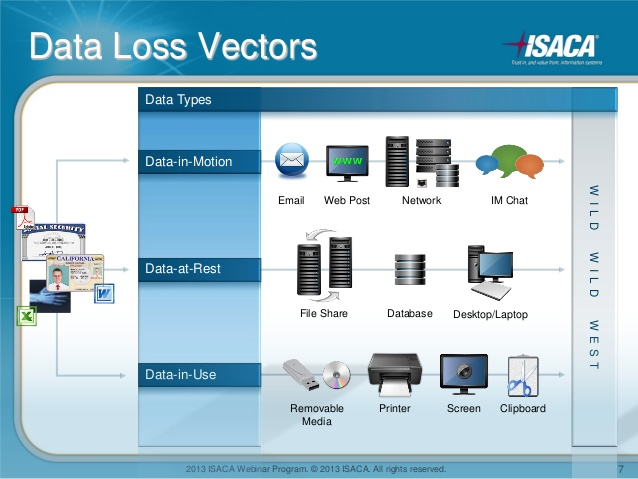
\includegraphics[width=.8\textwidth, height=.6\textheight, keepaspectratio]{data loss vectors.jpeg}}
        \caption{Modello ISACA: Data Loss Vectors}\label{ModelloIsaca}
      \end{figure}

\section{Accenni sul progetto}
Il progetto implementato consiste in una soluzione DLP per la protezione dei dati in transito, più precisamente per
l'identificazione di eventuali contenuti sensibili presenti nelle email aziendali, in modo da prevenirne la perdita
ed evitarne la diffusione.

Il confronto effettuato tra i prodotti principali presenti sul mercato, anche se nessuno di essi è stato utilizzato 
ai fini del progetto, è stato utile per capire quali caratteristiche dovesse possedere la soluzione DLP implementata.

\section{Tecnologie utilizzate}
Per l'implementazione del progetto sono state utilizzate diverse tecnologie:
    \subsection{Postfix}
    Postfix è un server di posta open source scritto in C da Wietse Zweitze Venema e distribuito con licenza IBM 
    Public License. Nasce alla fine degli anni '90 con lo scopo di fornire un'alternativa a Sendmail che offrisse 
    maggiori garanzie per quanto riguarda la sicurezza \cite{Postfix1}.
    Dato che il capitolo 5 si concentra esclusivamente su Postfix e come è stato utilizzato per implementare la 
    soluzione DLP, non spenderò altre parole per parlarne in questo paragrafo.
    
    \subsection{Python}
    Python è un linguaggio di programmazione di più alto livello che si presta ad essere utilizzato in ambito didattico per la sua semplicità. È orientato a oggetti, adatto, tra gli altri usi, a sviluppare 
    degli script \cite{Python1}. A differenza di linguaggi come il C e Java è un linguaggio interpretato e non compilato. 
    Il programma interprete di Python si occupa di tradurre le righe scritte in Python in istruzioni direttamente 
    comprensibili al computer (linguaggio macchina). I programmi scritti in Python sono portabili, 
    cioè possono essere eseguiti su differenti sistemi operativi, tra i quali Windows, Mac OS X e GNU/Linux. 
    Inoltre è gratuito e open source, utilizzabile da chiunque \cite{boscaini2017imparare}.

    
    \subsection{Bash}
    La Bash è la shell più diffusa e utilizzata in ambiente Linux. 
    Si tratta di un interprete di comandi che permette all'utente di comunicare col sistema operativo attraverso una
    serie di funzioni predefinite, o di eseguire programmi e script.
    Bash mette a disposizione un semplice linguaggio di scripting nativo che permette di svolgere compiti 
    più complessi, non solo raccogliendo in uno script una serie di comandi, 
    ma anche utilizzando variabili, funzioni e strutture di controllo di flusso \cite{Bash1}.
    
    \subsection{Apache Tika}
    Apache tika è un tool per l’analisi dei contenuti, permette di estrarre il testo da migliaia di tipi di file diversi \cite{tika}.
    Libreria utile per estrarre il testo dagli allegati delle email per verificare se contengono dati sensibili. 
    %Ho utilizzato questa libreria all’interno del mio script Python per estrapolare il testo dai file allegati 
    %alle email in modo da verificare la presenza di dati sensibili.
    
    \subsection{Virtualbox}
    Oracle VM VirtualBox è un software gratuito e open source per l'esecuzione di macchine virtuali \cite{VirtualBox1}.
    Attraverso l’uso di questo software ho potuto installare il sistema operativo CentOS 8 
    (distribuzione Linux derivata da Red Hat Enterprise Linux), che ha ospitato il mail server Postfix.